\documentclass{article}
\usepackage{neurips_2026}
\usepackage[utf8]{inputenc}
\usepackage[T1]{fontenc}
\usepackage{hyperref}
\usepackage{url}
\usepackage{booktabs}
\usepackage{amsfonts}
\usepackage{amsmath}
\usepackage{nicefrac}
\usepackage{microtype}
\usepackage{xcolor}
\usepackage{graphicx}
\graphicspath{{../figures/splicebert/workshop_edits/}{../figures/splicebert/}{../figures/origin-crossmodel/}}

\title{Mechanistic Discovery in Genomic Foundation Models:\\
How SpliceBERT Recognizes Splice Donors}

\author{Anonymous}

\newcommand{\Uinfo}{\ensuremath{U_{\mathrm{info}}}}

\begin{document}

\maketitle

\begin{abstract}
Genomic foundation models (GFMs) learn representations of DNA and RNA at scale, but the internal computations underlying their predictions are largely opaque. We apply mechanistic interpretability methods to SpliceBERT, a masked language model pretrained on primary RNA sequences from 72 vertebrate species, to trace how it predicts splice donors. We recover a structured causal circuit: attention head L3H1 combines a predominantly positional \emph{address} with an \emph{acceptor-local payload} and writes a low-rank donor-side representation (\Uinfo) that downstream heads transport to the masked-donor readout. Tracing the addressing mechanism reveals a learned period-3 positional carrier — a rank-2 Fourier component of the position-embedding matrix — that is causally required for donor--acceptor coupling ($0.946 \to 0.027$), absent from matched human-only and ORF-free ncRNA models, and confirmed by nucleotide-invariant phase surgery on 943 held-out genes ($\Psi_C = +0.141\ [0.110, 0.172]$ logit units). The carrier is an artifact of multi-species pretraining, not a human-sequence statistic — a discovery enabled by interpretability methods applied to a genomic model.
\end{abstract}

\section{Introduction}
\label{sec:intro}

Genomic foundation models achieve strong performance on RNA and DNA prediction tasks~\citep{chen2024splicebert,chen2022rnafm,akiyama2022rnabert}, but the computations they perform to reach those predictions are largely unknown. This opacity matters: these models encode evolutionary pressure across thousands of species and millions of sequences, and their internal representations may contain biological knowledge not accessible by behavioral probing alone.

Mechanistic interpretability~\citep{elhage2021framework} offers a path from behavior to mechanism. Instead of asking what a model \emph{knows}, it asks what computations it \emph{performs}, using causal interventions as the arbiter. Prior work in NLP has traced circuits for indirect object identification~\citep{wang2022ioi}, documented the information geometry of BERT representations~\citep{rogers2020bertology}, and developed automated circuit-discovery tools~\citep{conmy2023acdc}. Key methodological advances — reconstruct--inject patching~\citep{elhage2021framework}, subspace analysis~\citep{makelov2024subspace}, and activation patching decompositions~\citep{heimersheim2024patching} — have made circuit-level accounts tractable. However, no analogous mechanistic account exists for any genomic model.

We close this gap with SpliceBERT~\citep{chen2024splicebert}, an RNA masked language model pretrained on 72 vertebrate species. Using reconstruct--inject activation patching, QK/OV subspace analysis, and nucleotide-invariant causal surgery, we trace the computation underlying splice donor prediction. Our contributions are:
\begin{enumerate}
\item A complete circuit account — the address--payload--deliver structure that links donor recognition to its paired acceptor (§\ref{sec:circuit}).
\item Discovery and confirmation of a causally necessary, corpus-learned period-3 positional carrier absent from matched alternative models (§\ref{sec:carrier}).
\item Faithfulness quantification showing the identified core is a structured top-ranked set within an irreducibly distributed computation (§\ref{sec:faithfulness}).
\end{enumerate}

\section{Methods}
\label{sec:methods}

\subsection{Model and task}
SpliceBERT.1024nt is a post-LayerNorm BERT-style masked language model (6 layers, 16 heads, hidden size 512) with absolute learned position embeddings over $P=1026$ positions, pretrained on primary RNA sequences from 72 vertebrate species~\citep{chen2024splicebert}. We study \emph{masked donor prediction}: given a transcript with a splice donor masked, the model predicts the canonical GU dinucleotide. All experiments use canonical short introns from GENCODE v43~\citep{mudge2023gencode} with a fixed gene split (chr8/9 sealed test; held-out validation chr11/16/19; remaining chromosomes for discovery).

\subsection{Donor--acceptor coupling assay}
We measure coupling as the change in masked-donor MLM margin when the paired acceptor is corrupted (AG$\to$CC). Coupling is partner-specific ($+0.872\ [0.771, 0.969]$ logit units) and donor-specific, versus non-partner and other-donor controls ($+0.007/+0.005$), ruling out bulk sequence effects. The operator is validated as alt-invariant across six motif-hygienic dinucleotide substitutions within $\pm 25\%$ equivalence (planted-positive and permuted-label calibration both pass).

\subsection{Circuit tracing: reconstruct--inject and subspace analysis}
We use a \emph{reconstruct--inject} design: clean and corrupted residual streams are computed independently, then individual head or MLP activations are transplanted between them. Because SpliceBERT uses post-LayerNorm, QKV projections are linear in the layer-input residual, making transplants exact. We decompose L3H1's contribution into \emph{key/query address} and \emph{value payload} via a non-forced factorial intervention~\citep{heimersheim2024patching}. We identify \Uinfo\ (rank-8 left singular vectors of the clean-minus-corrupt final residual at the masked donor position) as a stable readout direction and verify it by held-out gene generalization.

\subsection{Position-table carrier analysis}
We extract the $P\times d$ learned position-embedding matrix and compute its Fourier power spectrum along the position axis to identify periodic components. For each candidate carrier band, we perform \emph{band deletion} (zeroing Fourier mass in the band) and measure effects on coupling and masked-base cross-entropy. Mediation tests use size-matched random-set nulls: a one-head restoration is scored only against random one-head sets.

\subsection{Phase surgery and origin comparison}
To confirm present-day carrier use free of nucleotide confounds, we apply \emph{nucleotide-invariant phase surgery}: for each gene, we shift the period-3 component of the position table by offsets $\{0,\ldots,9\}$ and measure coupling under each shift relative to 19 same-geometry hidden-axis controls (preserving Fourier support, Gram matrix, row norms, and perturbation RMS; changing only alignment with learned hidden features). To probe training origin, we compare carrier power between published-checkpoint sibling pairs: SpliceBERT.510nt (72 species) and SpliceBERT-human.510nt (human-only), sharing architecture, stage, and length, differing only in corpus. We additionally test RNA-FM and RNA-BERT~\citep{chen2022rnafm,akiyama2022rnabert} as ORF-free ncRNA comparators.

\section{Results}

\subsection{A structured address--payload--deliver circuit}
\label{sec:circuit}

Attention head L3H1 is the circuit keystone: ablating $\{$L3H1, L2H15$\}$ removes $81.6\%$ of coupling while retaining $99.2\%$ general MLM health. L3H1's contribution is conjunctive — key-only and value-only effects are small, whereas key+value gives $+0.663$ with interaction $+0.531\ [0.477, 0.583]$. This dissects into two separable streams (Figure~\ref{fig:circuit}A):

\paragraph{Address.} L3H1 attends to the paired acceptor based on position-embedding geometry, not acceptor sequence identity. The address is predominantly relative-offset based with modest absolute-position modulation. Head L2H15 amplifies the positional attraction through L3H1's address channel; the targeting advantage is already present in the embeddings and is amplified through layers 0--2.

\paragraph{Payload.} The acceptor-local state used by L3H1 is assembled by a serial generator: $\{$L0H7, L0H12, L0H10$\} \to$ MLP0 $\to$ MLP1 $\to$ MLP2. This payload is localized to the four-token acceptor window and is not explained by bulk GC content, polypyrimidine tract, or positional composition covariates. Its semantic identity is unresolved and must not be glossed as splice-site strength.

\paragraph{Delivery.} L3H1 writes a compact low-rank representation \Uinfo\ at the donor position: rank-8 recovery is $0.92$ versus random-subspace controls $\leq 0.05$. Restoring L3H1 recovers $0.83$ of coupling, $93\%$ of which routes through \Uinfo. Downstream transporter heads L4H0, L4H2, and L5H11 carry this state to the masked-donor MLM margin. The \Uinfo\ direction generalizes across gene-disjoint sets (rank-1 overlap $0.970$; held-out sufficiency $+0.875$), and cross-example injection transfers as a gene-generic readout axis.

\subsection{The period-3 positional carrier}
\label{sec:carrier}

Fourier analysis of SpliceBERT's $1026 \times 512$ position-embedding matrix reveals a rank-2 period-3 component ($289\times$ median band power; mean resultant length $0.977$). Deleting this band collapses donor--acceptor coupling from $0.946$ to $0.027$ while inflicting disproportionate damage on exon predictions ($+0.159$ nats) relative to introns ($+0.042$ nats). Restoring a single head (L2H15 or L3H1) after deletion recovers $36.3\%$/$34.8\%$ of coupling, well above the best one-head random null of $4.2\%$. The carrier acts as a distributed relative-positional addressing clock, recovered mainly through L3H1's attention pattern rather than carrier-dependent changes in its values ($+0.284$ vs.\ $-0.005$ confirm).

\paragraph{Phase surgery confirms phase-aligned causal use.} Nucleotide-invariant local phase shifts applied to 943 held-out genes show that off-register shifts ($\{1,2,4,5,7,8\}$) reduce coupling selectively inside CDS blocks, while in-register shifts ($\{3,6,9\}$) preserve it (Figure~\ref{fig:surgery}). The preregistered primary estimand — CDS modulo-recovery minus upstream-intron modulo-recovery — is $\Psi_C = +0.141\ [0.110, 0.172]$ logit units, exceeding the frozen SESOI of $0.05$. The learned period-3 direction exceeds all 19 same-geometry hidden-axis controls (Figure~\ref{fig:surgery}C); paired excess $+0.136\ [0.051, 0.222]$, exact add-one $p = 0.05$. The matched CDS-minus-non-CDS-exon contrast is $+0.006\ [-0.080, +0.093]$ (Figure~\ref{fig:surgery}D) — inconclusive for coding enrichment.

\paragraph{Corpus origin.} The carrier is strong in the 72-species stage-1 checkpoint ($435\times$ median band power) and undetected in its human-only sibling ($6.2\times$; permutation $p = 0.071$; ratio $70\times$). The $\approx\!10.63$-nt carrier shows an even larger contrast ($369\times$ vs.\ $2.4\times$; ratio $153\times$). Both carriers are absent from RNA-FM and RNA-BERT, trained on ORF-free ncRNA, under powered nulls. A model-free spectral scan finds no $\approx\!10.63$ periodicity in $60$~Mb of human genome. The period-3 carrier is therefore an artifact of multi-species pretraining rather than a reflection of any human-sequence statistic.

\subsection{Faithfulness and distributional structure}
\label{sec:faithfulness}

We measure \emph{complement faithfulness}: the fraction of coupling preserved when only nodes outside the named circuit are active. The named spine is necessary ($N = 0.989$) and sufficient when injected ($D = 0.986$), but fails as a standalone sparse generator ($F = 0.005$). A held-out complement-faithfulness size curve (Figure~\ref{fig:circuit}B) rises gradually and crosses $90\%$ only near $72$ of $103$ nodes, with no sparse knee. The named components form a \emph{structured causal core within an irreducibly distributed computation} — not the complete generator. Minimality is unclaimed.

\begin{figure}[t]
  \centering
  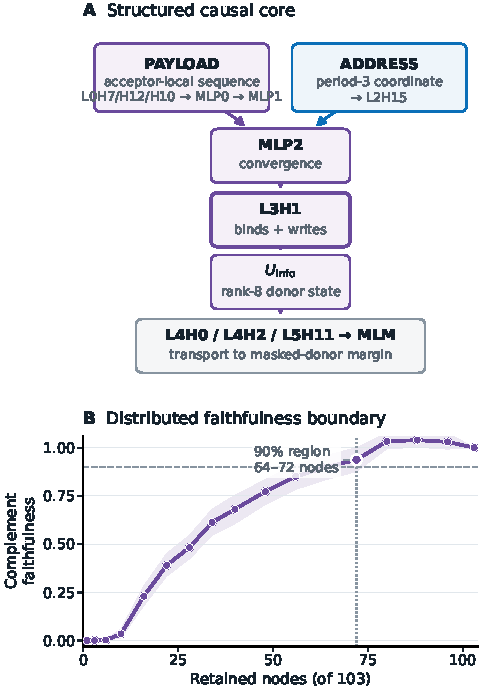
\includegraphics[width=\linewidth]{fig_full_circuit_edit.pdf}
  \caption{\textbf{Structured donor--acceptor core and its faithfulness boundary.}
  \textbf{(A)} The acceptor-local value payload (assembled by L0H7/H12/H10 and the MLP0$\to$MLP1 backbone) and the predominantly positional address (period-3 carrier via L2H15) converge through MLP2 at L3H1, which writes the rank-8 donor-side readout state \Uinfo. Transporter heads L4H0, L4H2, and L5H11 carry \Uinfo\ to the masked-donor MLM margin.
  \textbf{(B)} Held-out complement faithfulness rises gradually; the sampled $90\%$ crossing lies between 64 and 72 of 103 nodes with no sparse knee. The named mechanism is a structured top-ranked core inside a broad interaction-dependent computation.}
  \label{fig:circuit}
\end{figure}

\begin{figure}[t]
  \centering
  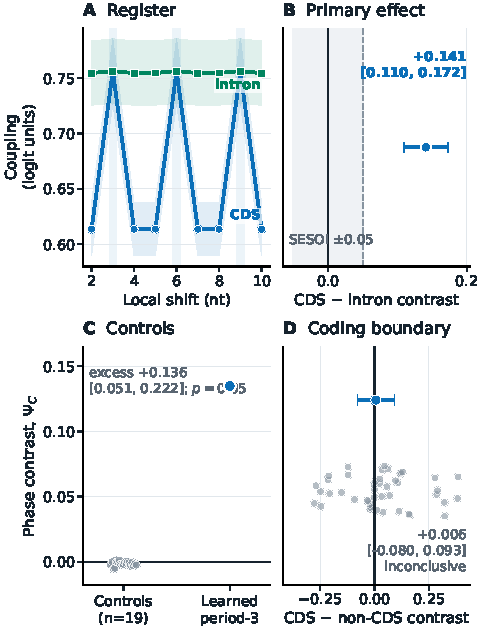
\includegraphics[width=\linewidth]{fig5_p3_phase_surgery_confirmation_edit.pdf}
  \caption{\textbf{Nucleotide-invariant surgery confirms phase-aligned period-3 use.}
  \textbf{(A)} Mean donor--acceptor coupling under local period-3 phase shifts. Off-register shifts reduce coupling inside CDS blocks but not under the matched upstream-intron control. Ribbons are $\pm 1$ gene-level SE (descriptive).
  \textbf{(B)} The preregistered estimand $\Psi_C$ (CDS minus upstream-intron modulo-recovery) is $+0.141\ [0.110, 0.172]$ across $n=943$ genes, exceeding the frozen SESOI ($0.05$).
  \textbf{(C)} The learned period-3 direction exceeds all 19 same-geometry hidden-axis controls; paired learned-minus-control excess $+0.136\ [0.051, 0.222]$, $p=0.05$.
  \textbf{(D)} The CDS-minus-non-CDS-exon contrast ($+0.006\ [-0.080, +0.093]$) is inconclusive; coding enrichment is not established.}
  \label{fig:surgery}
\end{figure}

\section{Discussion}

\paragraph{The period-3 carrier as an interpretability discovery.}
The carrier would not surface in a behavioral analysis of SpliceBERT's outputs: it is causally required for donor--acceptor coupling, but coupling itself is not the pretraining objective. Discovering it required examining the Fourier geometry of the absolute position-embedding matrix and following the causal chain through to behavior. The corpus-comparison experiment then showed that the carrier is a multi-species training artifact, suggesting that period-3 statistics in the vertebrate transcriptome — plausibly codon-period signal in CDS regions — were distilled into the position table during pretraining. Whether this periodicity corresponds to any biologically meaningful feature beyond codon phasing is now a tractable question that mechanistic interpretability has opened.

\paragraph{Irreducible distribution in a small model.}
The faithfulness curve's lack of a sparse knee — in a 6-layer, 96-head model with only one behavioral target — challenges the assumption that mechanistically identified circuits are sparse generators. The named components are causally well-supported and necessary, but the broad distributed remainder is load-bearing. Applications of circuit methods to larger GFMs should anticipate this: the interesting causal structure may be real and well-localized, while still not being a faithful standalone generator.

\paragraph{Open questions.}
Three questions remain structurally open at the model level. First, the payload's semantic identity: acceptor-local, resistant to compositional covariates, but not nameable without training-time interventions or external splice-assay data. Second, the $\approx\!10.63$-nt carrier: it routes through eight heads post-softmax, its donor-coupling contribution is bounded at $-0.033\ [-0.061, -0.005]$ logit units (small and suppressive), and its general OV function is open. Third, cross-example acceptor-payload specificity is not separable at current precision. These open questions have direct analogues in NLP mech interp (payload identity $\sim$ feature identification; distributional structure $\sim$ polysemanticity), suggesting the methodological toolkit is shared even when the biological substrate introduces new complexity.

\section{Conclusion}

We present the first mechanistic circuit account for a genomic foundation model, tracing how SpliceBERT implements splice donor recognition through a structured address--payload--deliver circuit mediated by L3H1. The period-3 positional carrier — discovered through position-table Fourier analysis, causally confirmed by nucleotide-invariant surgery, and comparatively attributed to multi-species pretraining — demonstrates that mechanistic interpretability can surface novel knowledge about what genomic models learn and why. The approach is not SpliceBERT-specific; reconstruct--inject patching and position-table analysis should transfer to any post-LayerNorm transformer GFM with absolute position embeddings.

\bibliography{refs}
\bibliographystyle{plainnat}

%% NeurIPS 2026 Workshop Paper Checklist
%% Interpretability for Discovery Workshop

\section*{Paper Checklist}

\begin{enumerate}

\item \textbf{Claims.}
Do the main claims made in the abstract and introduction accurately reflect the paper's contributions and scope?
\answerYes{} The abstract and introduction present three specific claims (circuit structure, period-3 carrier, faithfulness) that are directly supported by the results in §3. Each claim is scoped to one checkpoint (SpliceBERT.1024nt), one task (masked donor prediction), and one behavioral assay (canonical short introns). No transfer to biological mechanisms or other models is asserted beyond what is measured.

\item \textbf{Limitations.}
Did you discuss the limitations of your work?
\answerYes{} §4 (Discussion) explicitly identifies three open questions: (a) the acceptor-payload semantic identity is unresolved and cannot be named on the current checkpoint; (b) the $\approx$10.63-nt carrier's OV function in the donor circuit is bounded at sub-SESOI levels and its general function is open; (c) cross-example specificity of the acceptor payload is not separable at current precision. §3.3 clarifies that the named circuit is a structured core within an irreducibly distributed computation, not a minimal sparse generator.

\item \textbf{Theory assumptions and proofs.}
If the paper includes theoretical contributions, do all theorems, corollaries, etc.\ appear to be correct?
\answerNA{} This paper contains no theoretical claims or proofs.

\item \textbf{Experimental reproducibility.}
Are the experimental results reproducible?
\answerYes{} All results are derived from the published SpliceBERT checkpoint (publicly available) and GENCODE v43 annotations (public). Code, preregistrations, and JSON result artifacts are included in the supplementary repository. Every claim is controlled by an immutable artifact file listed in the results manifest. Pre-registered protocols with smoke-gate tests and adversarial verification were used throughout.

\item \textbf{Code.}
Is code available, or will it be made available?
\answerYes{} The full analysis codebase will be released upon de-anonymization. The codebase includes all runner scripts, pre-registration documents, and result manifests.

\item \textbf{Compute.}
Does the paper include the compute required to reproduce the results?
\answerYes{} All experiments use a single pre-trained SpliceBERT checkpoint (inference only, no training). Compute requirements are modest: all analyses run on a single GPU in under 48 hours total. No large-scale compute is required to reproduce these results.

\item \textbf{Data.}
Does the paper reference all data used?
\answerYes{} The model (SpliceBERT.1024nt) is publicly available~\citep{chen2024splicebert}. Genomic annotations use GENCODE v43~\citep{mudge2023gencode}. RNA-FM and RNA-BERT checkpoints are publicly available~\citep{chen2022rnafm,akiyama2022rnabert}. The human-only SpliceBERT sibling checkpoint is publicly available from the same source as SpliceBERT.

\item \textbf{IRB approvals.}
If the paper involves human subjects, was ethical approval obtained?
\answerNA{} This paper involves no human subjects. All data are publicly available genomic annotations and pre-trained model weights.

\item \textbf{Responsible use.}
Does the paper discuss potential positive societal impacts, as well as any potential negative impacts?
\answerYes{} See below.

\end{enumerate}

\subsection*{Responsible Use Statement}

\paragraph{Potential positive societal impacts.}
This work develops mechanistic interpretability methods applicable to genomic foundation models. The methods — reconstruct--inject patching, position-table Fourier analysis, and nucleotide-invariant causal surgery — are designed to surface internal computations that are not accessible by behavioral probing alone. Positive impacts include: (1) improved understanding of what genomic models learn from multi-species pretraining data; (2) a transferable methodological template for auditing other GFMs for spurious or biologically meaningful features; (3) identification of open questions (e.g.\ acceptor-payload identity) that can guide future model evaluation and data collection.

\paragraph{Potential risks and mitigations.}
The methods described in this paper are interpretability tools applied to an existing published model; they do not enable training new genomic models or generating novel sequences. The primary risk is misinterpretation of results: (1) the donor--acceptor circuit is a model mechanism, not a direct claim about spliceosome biochemistry or transcript abundance; no external biological assay is used; (2) the period-3 carrier is attributed to multi-species pretraining by comparative analysis, not by retraining — origin dynamics cannot be recovered from a single checkpoint; (3) the faithfulness results show the named circuit is not a minimal sparse generator, and minimality is explicitly unclaimed. We have taken care throughout to scope claims precisely (see §3 and §4) and to avoid overstating biological implications. The open-source release of code and preregistration documents will allow independent verification and replication.

\paragraph{Broader context.}
Genomic foundation models are increasingly used in research and clinical genomics contexts. Mechanistic interpretability provides a tool for auditing these models before deployment, identifying features that may be spurious artifacts of training data rather than reflections of underlying biology. We view this work as a step toward model transparency in a domain where the stakes of misinterpreted predictions are high.


\end{document}
